\documentclass[t, 10pt, aspectratio=1610]{beamer}
 % align text inside frame to t=top, b=bottom, c=center
 % 8pt, 9pt, 10pt, 11pt, 12pt, 14pt, 17pt, 20pt available as text font
 % select your aspect ratio 4:3=43, 16:9=169, 16:10=1610

\usetheme{Juelich}

%\usetheme{default}
%\usecolortheme{beaver}

\setbeamertemplate{caption}[numbered]
\setbeamertemplate{caption label separator}{:}
\setbeamertemplate{slide counter}[showall]
\setbeamercolor{code}{fg=black,bg=fzjblue!10}
\setbeamercolor{prototype}{fg=black,bg=fzjgreen!20}

% \setbeamertemplate{footer element1}[default][\insertsection]%

\newcommand{\activatefootline}{
\setbeamertemplate{footline}
{
    \leavevmode%
    \hbox{%
        \begin{beamercolorbox}[wd=\paperwidth,ht=0.25ex,dp=1ex,right]{date in head/foot}%
            \usebeamerfont{author in head/foot}\insertauthor\hspace*{2em}
            \insertframenumber{}\hspace*{2ex}
        \end{beamercolorbox}}%
        \vskip0pt%
}
}

\newcommand{\deactivatefootline}{\setbeamertemplate{footline}{}}

\usepackage{graphics}
\newcommand{\gfxpath}{../images}

\usepackage[ngerman,english]{babel}
%\selectlanguage{ngerman}
\selectlanguage{english}
\usepackage[utf8]{inputenc}
\usepackage[T1]{fontenc}
% =====================================================
%  packages / definitions needed by pandoc
%
\usepackage{xcolor}
\usepackage{fancyvrb}
\usepackage{framed}
\usepackage{longtable}
\usepackage{booktabs}
\usepackage[warn]{textcomp}
% package listings important for code highlighting !
\usepackage{listings}

% for image placing
\usepackage{tikz}
\usetikzlibrary{calc}

\providecommand{\tightlist}{%
  \setlength{\itemsep}{0pt}\setlength{\parskip}{0pt}}

%\renewcommand{\emph}[1]{\structure{#1}}

\renewcommand{\thefootnote}{}

% AUTHOR AND TITLE FOR TITLE PAGE
\author[J. Jitsev]{Jenia Jitsev}
\institute[JSC]{Scalable Learning \& Multi-Purpose AI Lab, Helmholtz AI, LAION @ JSC}
\date{2023-05-09}
\title{Day 2: Towards Scalable Deep Learning}
\subtitle{Distributed Training and Data Parallelism}

%\AtBeginPart{%
%  \subtitle{\partname}
%  \makepart
%  \begin{frame}
%  \frametitle{Outline}
%  \tableofcontents[hideallsubsection]
%  \end{frame}
%}

%\AtBeginSection{%
%  \subtitle{\sectionname}
%  \begin{frame}
%  \frametitle{Outline}
%  \tableofcontents[currentsection]
%  \end{frame}
%}

% -- INCLUDE BACKGROUND GRAPHIC FOR TITLE PAGE
\titlegraphic{
\includegraphics[width=\paperwidth]{../images/placeholder}}


\begin{document}
% Titelseite
\fzjset{title page=image}

%\fzjset{title page=text}
\deactivatefootline
\maketitle

%\begin{frame}
%  \frametitle{Outline}
%  \tableofcontents
%\end{frame}

%% pandoc generated slides
\activatefootline
\begin{frame}
\end{frame}

\begin{frame}{Distributed Training on Large Data}
\protect\hypertarget{distributed-training-on-large-data}{}
\begin{itemize}
\tightlist
\item
  ImageNet-1k : still gold standard in training large visual recognition
  models
\item
  Serves as ``Hello World'' for large dataset training
\end{itemize}

\center{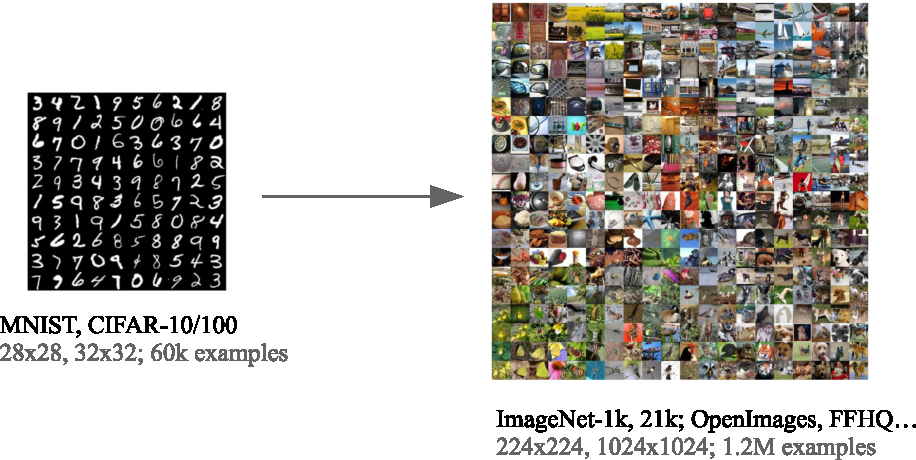
\includegraphics[width=0.8\textwidth]{../images/MNIST_CIFAR_ImageNet_Transition_Test.pdf}}
\end{frame}

\begin{frame}{Distributed Training on Large Data}
\protect\hypertarget{distributed-training-on-large-data-1}{}
\begin{itemize}
\tightlist
\item
  ImageNet-1k : still gold standard in training large visual recognition
  models
\item
  ResNet-50 : baseline model network, test accuracies : \(\approx 75\%\)
  top-1, \(\approx 94\%\) top-5 (Winner ILSVRC 2015)
\end{itemize}

\center{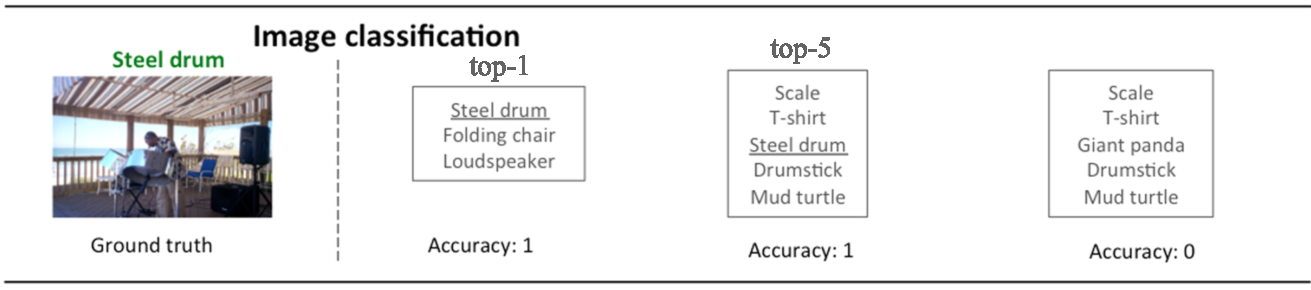
\includegraphics[width=0.8\textwidth]{../images/ImageNet_Accuracy_Detection_Top_Only_Test.pdf}}

\footnote<.->{\tiny Russakovsky et al, IJCV, 2015}
\end{frame}

\begin{frame}{Distributed Training on Large Data}
\protect\hypertarget{distributed-training-on-large-data-2}{}
\begin{itemize}
\tightlist
\item
  ResNets on ImageNet : efficient distributed training in data parallel
  mode possible

  \begin{itemize}
  \tightlist
  \item
    prerequisite is good scaling of throughput during training
  \item
    image throughput during training ideally increasing as
    \(\tau_K = K \cdot \tau_{ref}\) Images/sec
  \item
    training with a large effective batch size
    \(\vert \mathfrak{B} \vert = K \cdot \vert B_{\text{ref}} \vert\),
    \(K\) workers
  \end{itemize}
\end{itemize}

\center{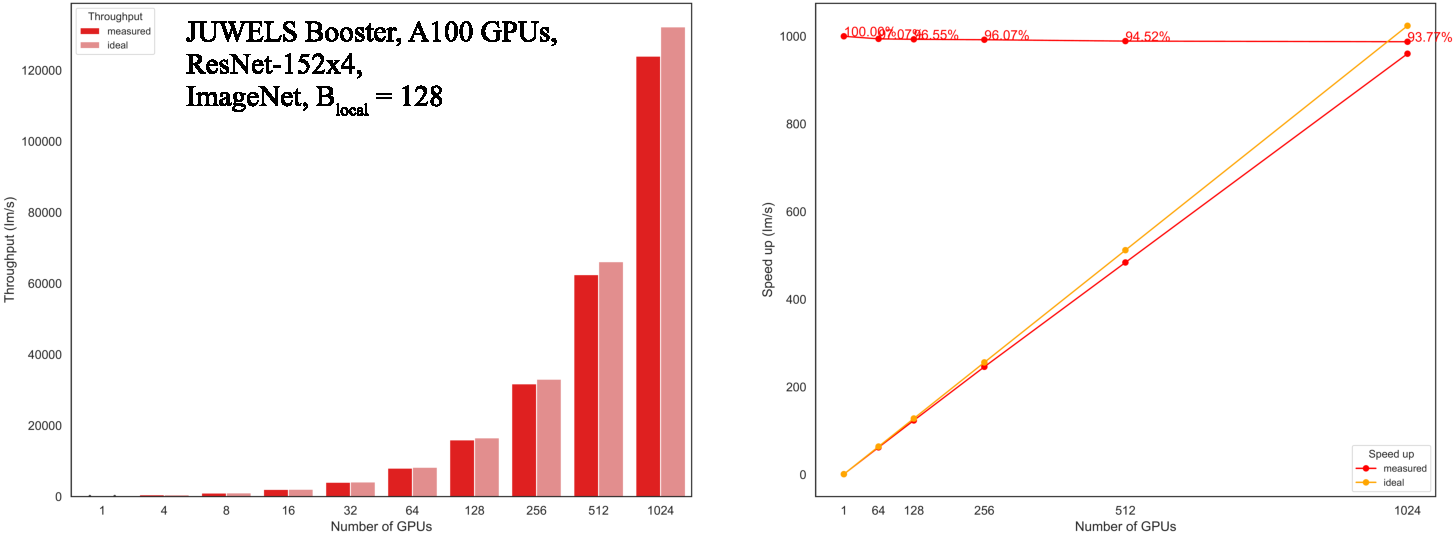
\includegraphics[width=0.9\textwidth]{../images/JUWELS_Booster_Ims_SpeedUp_ResNet-152x4_mod.pdf}}

\footnote<.->{\tiny Cherti and Jitsev, arXiv:2106.00116, MedNeurIPS
  Workshop, 2021}
\end{frame}

\begin{frame}{Distributed Training on Large Data}
\protect\hypertarget{distributed-training-on-large-data-3}{}
\begin{itemize}
\tightlist
\item
  ResNets on ImageNet : efficient distributed training in data parallel
  mode

  \begin{itemize}
  \tightlist
  \item
    High test accuracy in the end of the training is the goal
  \end{itemize}
\end{itemize}

\center{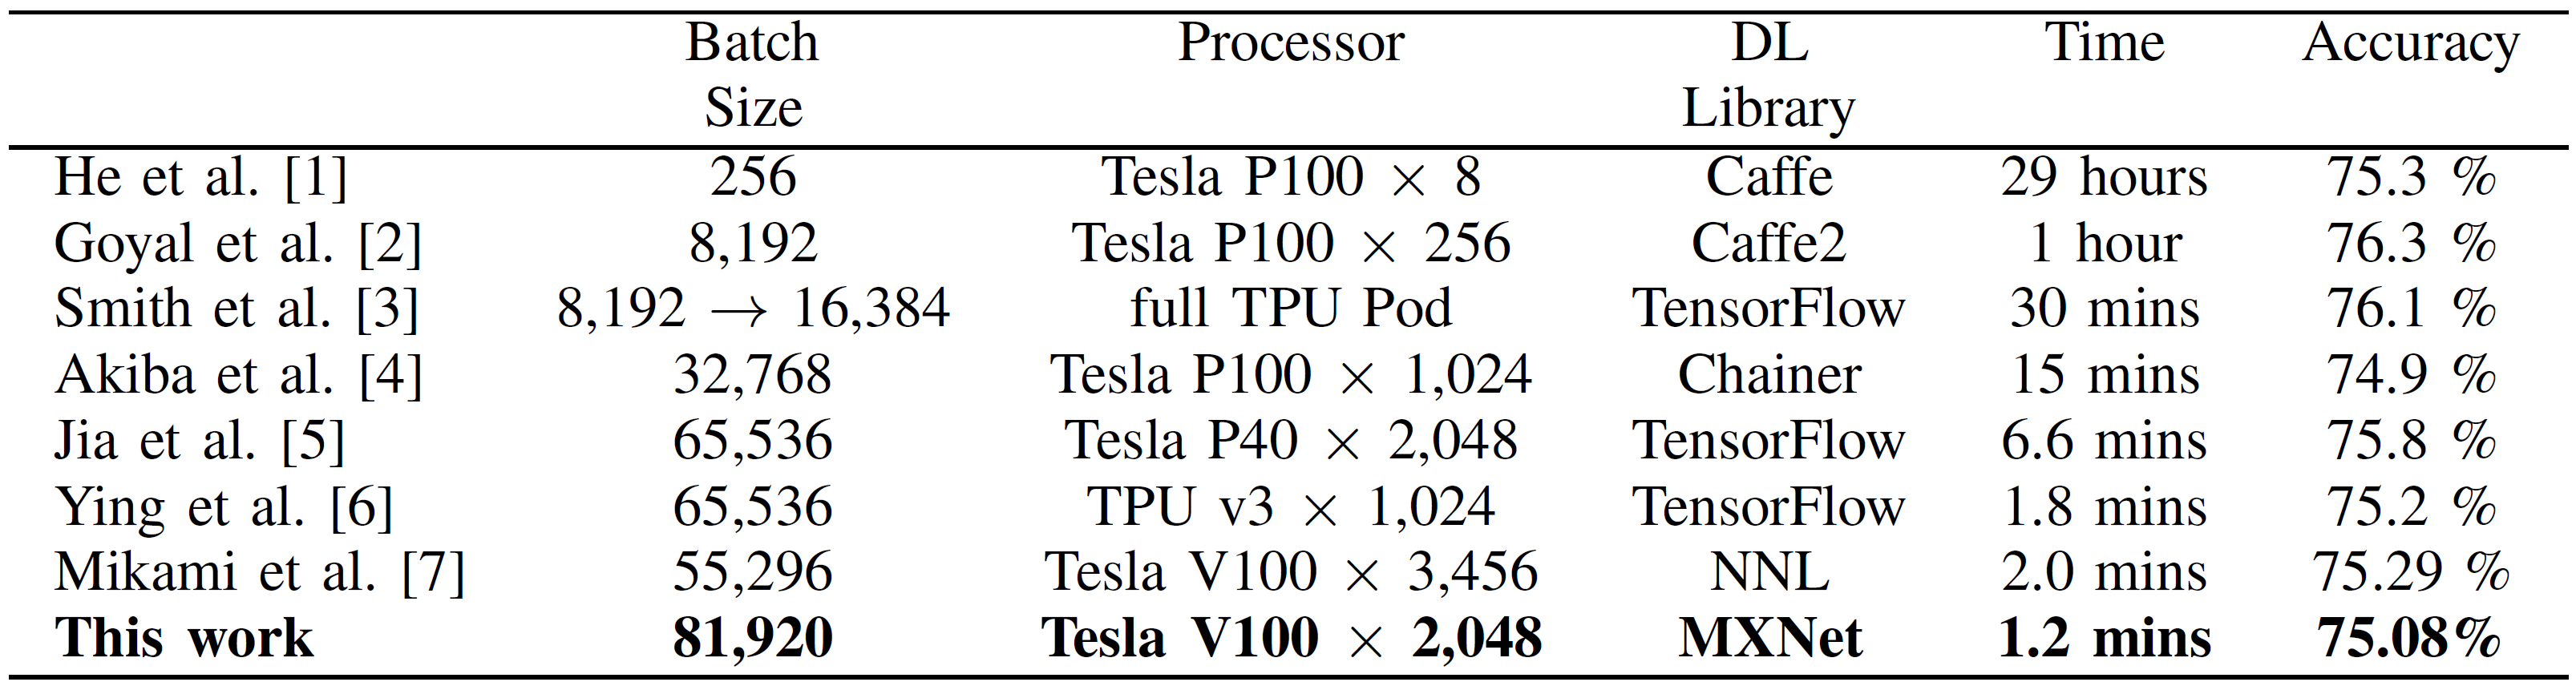
\includegraphics[width=0.6\textwidth]{../images/Yamazaki_RunTime_Table_ImageNet_ResNet-50_Accuracies.png}}

\center{ \hspace*{5cm} 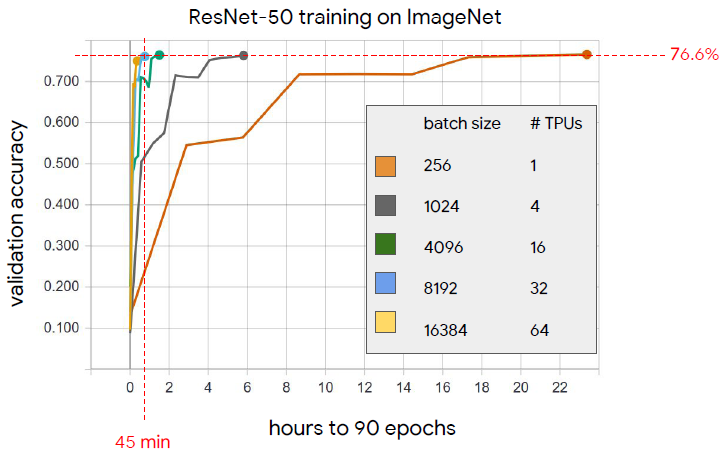
\includegraphics[width=0.4\textwidth]{../images/ResNet-50_ImageNet_Training_Time_Validation_Accuracy.png}}

\vspace*{-1cm}

\footnote<.->{\tiny Yamazoto et al, 2019; Ying, 2018}
\end{frame}

\begin{frame}{Distributed Training on Large Data}
\protect\hypertarget{distributed-training-on-large-data-4}{}
\begin{itemize}
\tightlist
\item
  Data parallel training: working with large effective batch sizes
\item
  Reminder: Training with
  \(\vert \mathfrak{B} \vert = K \cdot \vert B_{\text{ref}} \vert\),
  \(K\) workers
\item
  Large effective batch sizes alter model optimization trajectory
\end{itemize}

\center{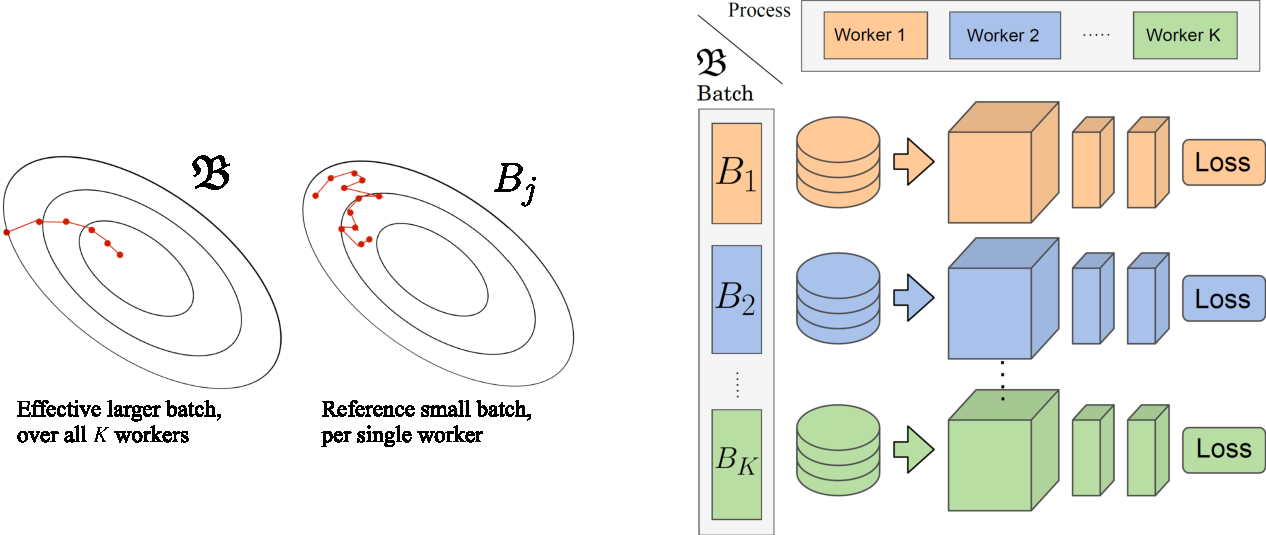
\includegraphics[width=0.9\textwidth]{../images/Large_Small_Reference_Batch_Data_Parallel_Model_Workers_Processes.pdf}}
\end{frame}

\begin{frame}{Distributed Training on Large Data}
\protect\hypertarget{distributed-training-on-large-data-5}{}
\begin{itemize}
\tightlist
\item
  Data parallel training: working with large effective batch sizes
\item
  Training with
  \(\vert \mathfrak{B} \vert = K \cdot \vert B_{\text{ref}} \vert\),
  \(K\) workers
\item
  Large effective batch sizes alter model optimization trajectory

  \begin{itemize}
  \tightlist
  \item
    may require hyperparameter re-tuning compared to a working smaller
    batch (single node) version
  \end{itemize}
\end{itemize}

\center{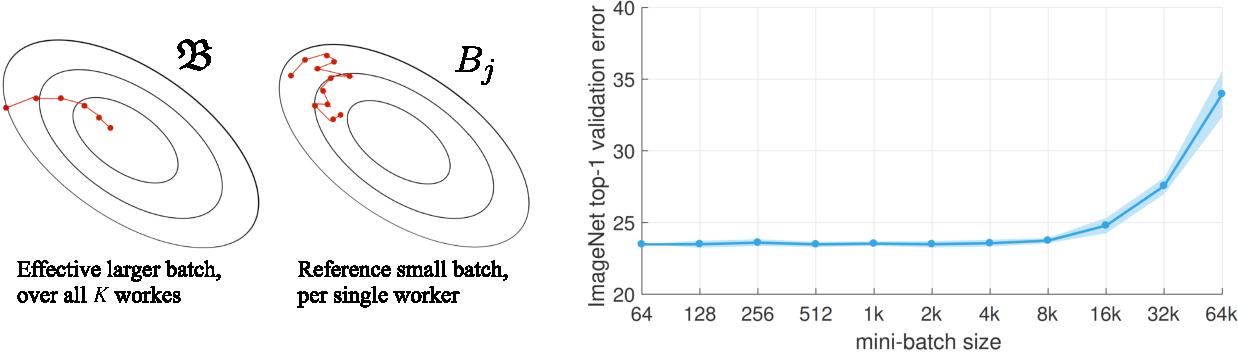
\includegraphics[width=0.8\textwidth]{../images/Effective_Reference_Batch_ImageNet_Goyal_2.pdf}}

\footnote<.->{\tiny Goyal et al, 2017}
\end{frame}

\begin{frame}{Distributed Training on Large Data}
\protect\hypertarget{distributed-training-on-large-data-6}{}
\begin{itemize}
\tightlist
\item
  ResNet-50 : efficient distributed training in data parallel mode

  \begin{itemize}
  \tightlist
  \item
    for very large batch sizes \(\vert \mathfrak{B} \vert\): diminishing
    speed-up returns when training towards a given test accuracy
  \end{itemize}
\end{itemize}

\center{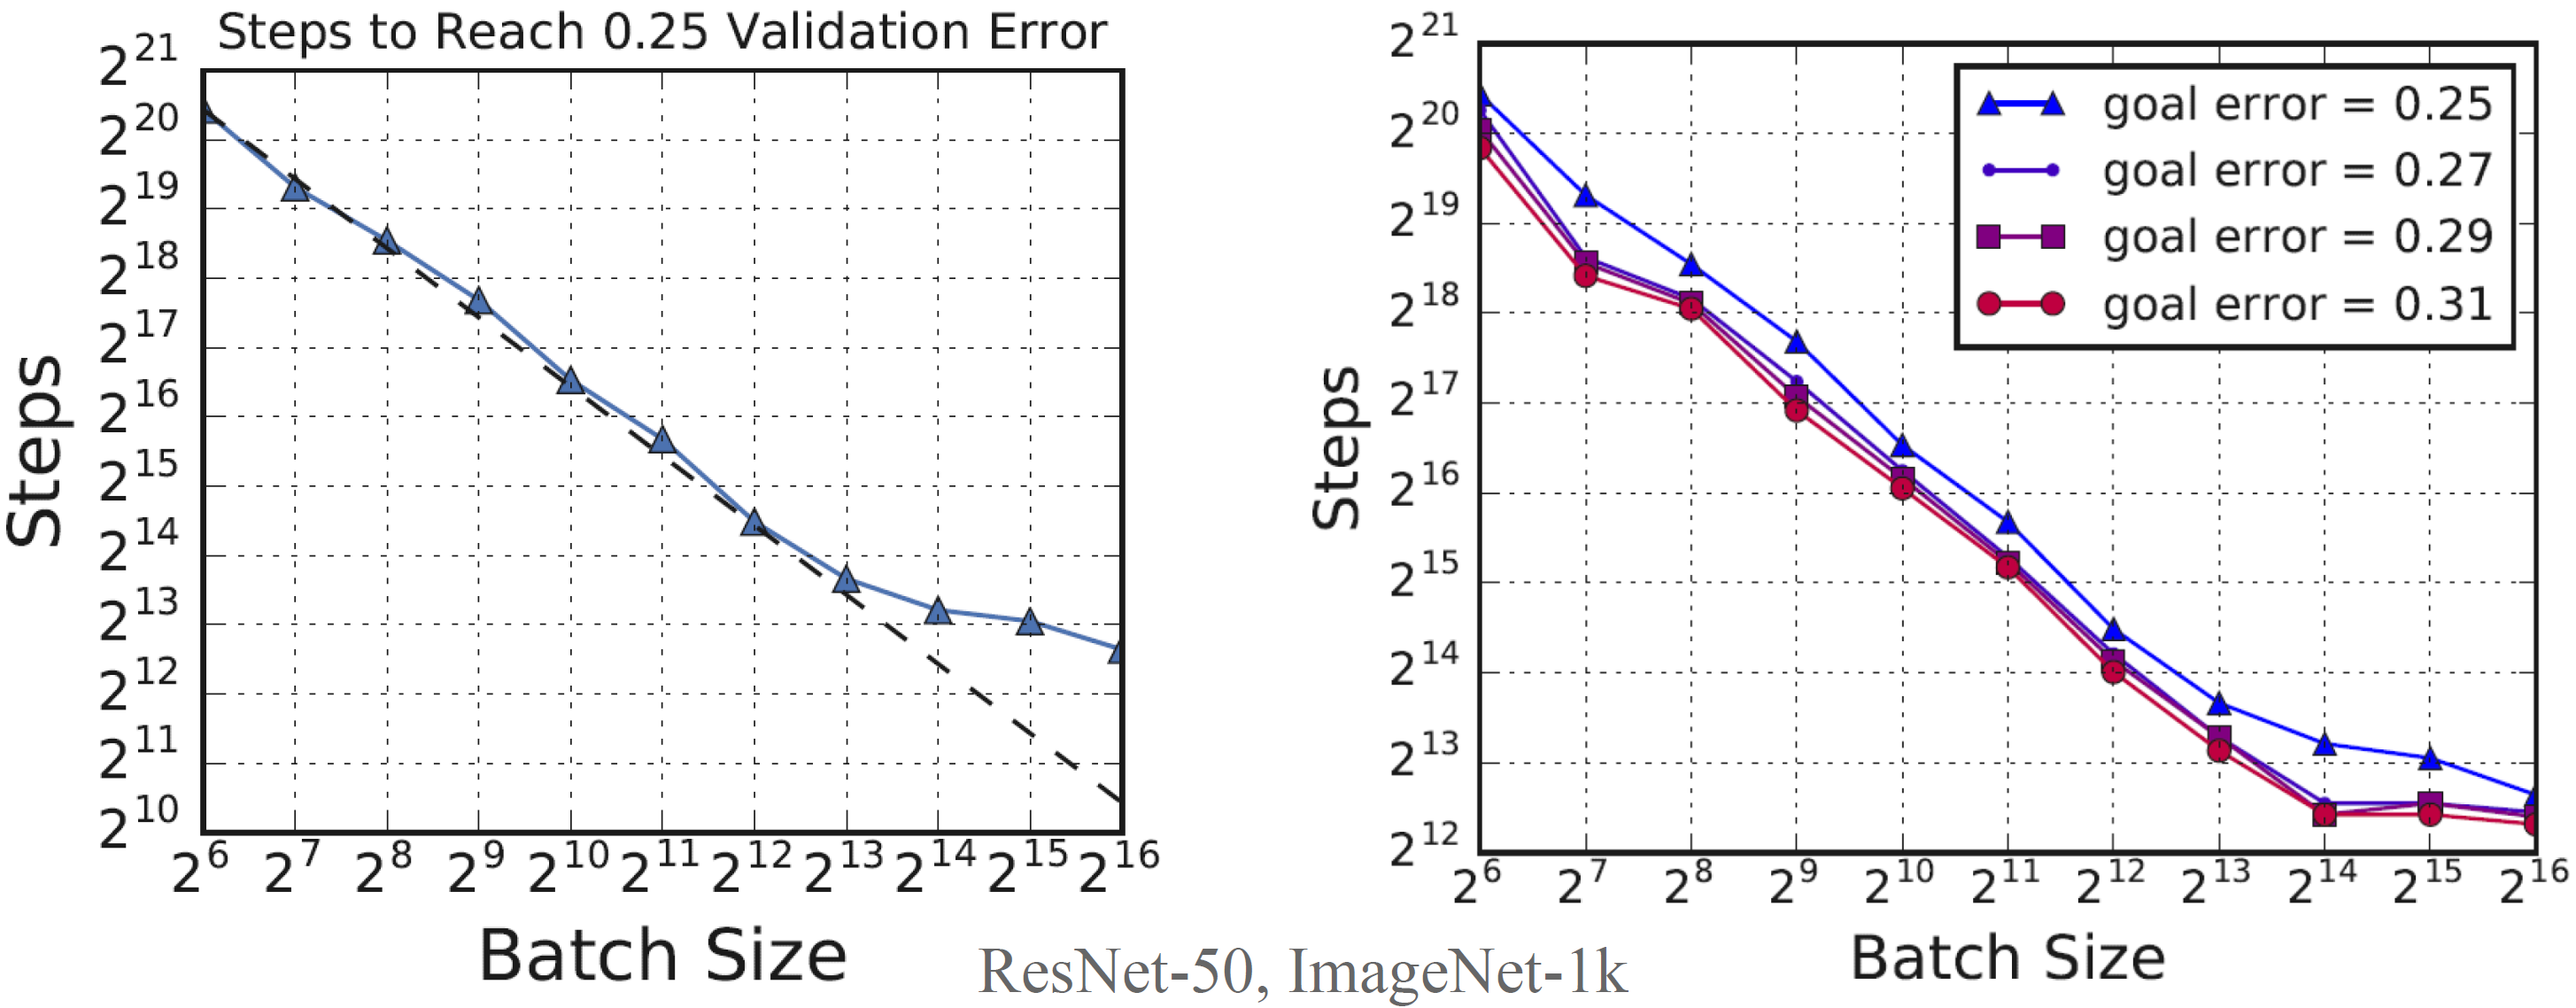
\includegraphics[width=0.8\textwidth]{../images/Batch_Size_Critical_ImageNet_ResNet-50_Goal_Error.png}}

\footnote<.->{\tiny Shallue et al, JMLR, 2019}
\end{frame}

\begin{frame}{Distributed Training on Large Data}
\protect\hypertarget{distributed-training-on-large-data-7}{}
\begin{itemize}
\tightlist
\item
  Critical large batch sizes \(\vert \mathfrak{B}_{\text{crit}} \vert\):
  diminishing speed-up when crossing, given target test accuracy
\end{itemize}

\center{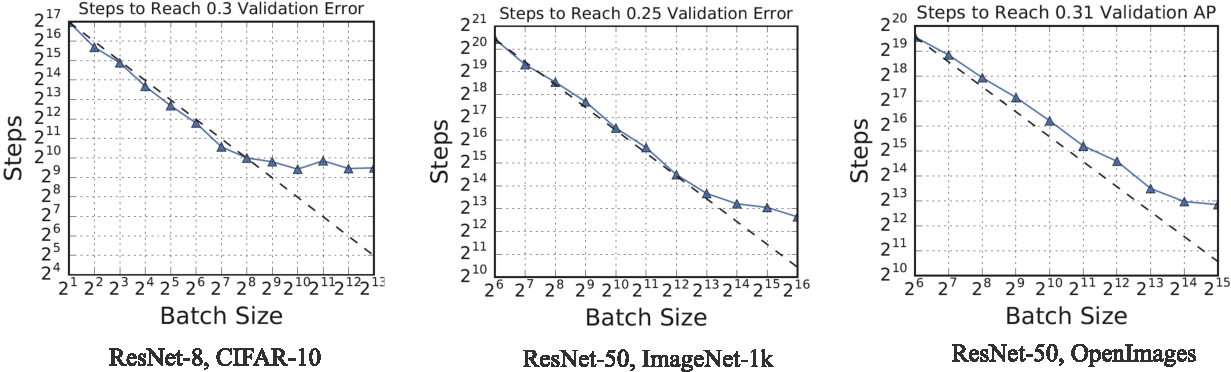
\includegraphics[width=\textwidth]{../images/Batch_Size_Critical_ResNet_Different_Datasets_Test.pdf}}

\footnote<.->{\tiny Shallue et al, JMLR, 2019}
\end{frame}

\begin{frame}{Distributed Training on Large Data}
\protect\hypertarget{distributed-training-on-large-data-8}{}
\begin{itemize}
\tightlist
\item
  Critical large batch sizes \(\vert \mathfrak{B}_{\text{crit}} \vert\):
  systematic evidence across datasets, tasks and architectures
\end{itemize}

\center{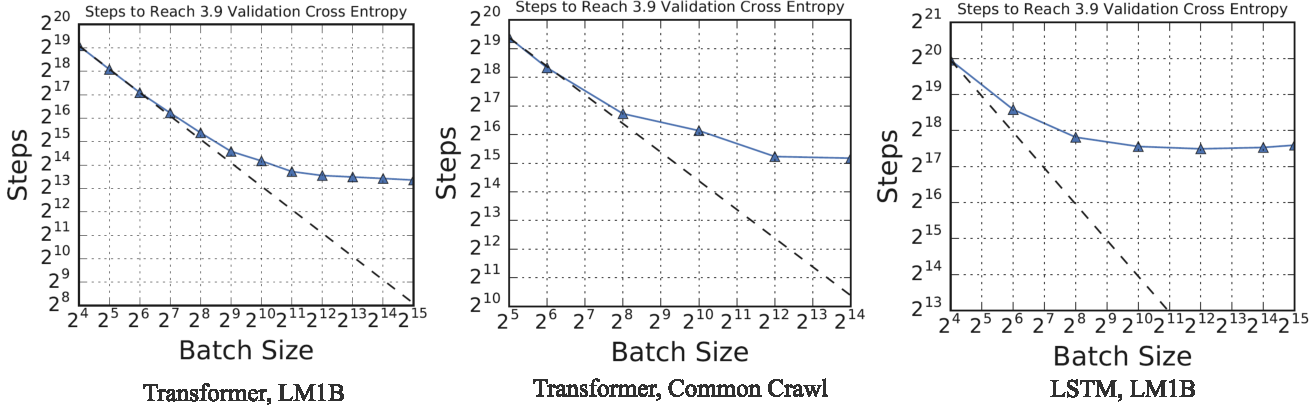
\includegraphics[width=\textwidth]{../images/Batch_Size_Critical_Transformer_Different_Datasets.pdf}}

\footnote<.->{\tiny Shallue et al, JMLR, 2019}
\end{frame}

\begin{frame}{Distributed Training on Large Data}
\protect\hypertarget{distributed-training-on-large-data-9}{}
\begin{itemize}
\tightlist
\item
  Critical large batch sizes \(\vert \mathfrak{B}_{\text{crit}} \vert\):
  large enough to do efficient distributed training
\item
  Efficient Distributed Training with
  \(\vert \mathfrak{B} \vert = K \cdot \vert B_{\text{ref}} \vert\), for
  large \(K\)

  \begin{itemize}
  \tightlist
  \item
    providing almost linear training speed up,
    \(t_{\mathfrak{B}} = \tfrac{1}{K} t_{B}\)
  \end{itemize}
\end{itemize}

\center{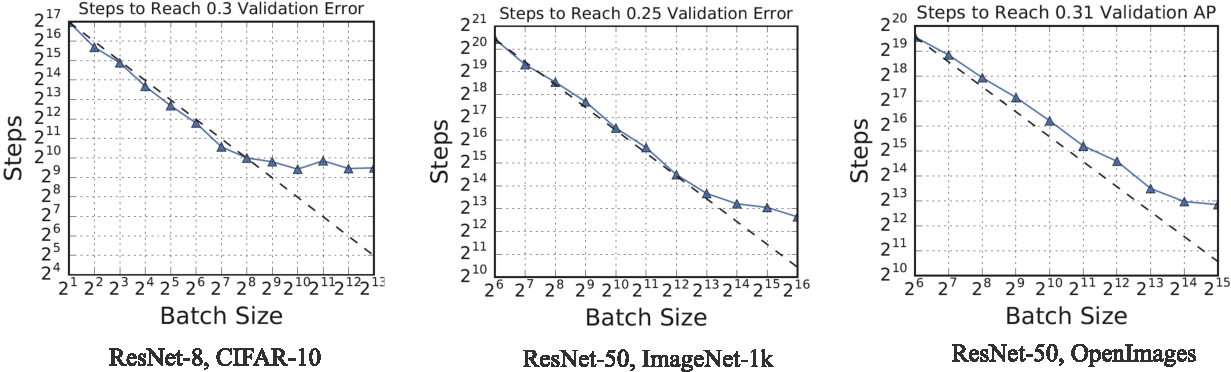
\includegraphics[width=\textwidth]{../images/Batch_Size_Critical_ResNet_Different_Datasets_Test.pdf}}

\footnote<.->{\tiny Shallue et al, JMLR, 2019}
\end{frame}

\begin{frame}{Distributed Training on Large Data}
\protect\hypertarget{distributed-training-on-large-data-10}{}
\begin{itemize}
\tightlist
\item
  Efficient Distributed Training with
  \(\vert \mathfrak{B} \vert = K \cdot \vert B_{\text{ref}} \vert\), for
  large \(K\)
\item
  Providing almost linear training speed up,
  \(t_{\mathfrak{B}} = \tfrac{1}{K} t_{B}\), \textbf{without loss of
  test accuracy}
\item
  Important: reducing training \textbf{time to accuracy} - \textbf{time
  to solution}

  \begin{itemize}
  \tightlist
  \item
    strong scaling : reducing \textbf{time to accuracy}
  \item
    reducing time per update step, per epoch, increasing samples
    throughput - alone not \textbf{sufficient} for speeding-up, reducing
    \textbf{time to accuracy}!
  \item
    doing ``bad'' update steps during training would require doing a lot
    of them before reaching target loss/accuracy \ldots{}
  \end{itemize}
\end{itemize}

\center{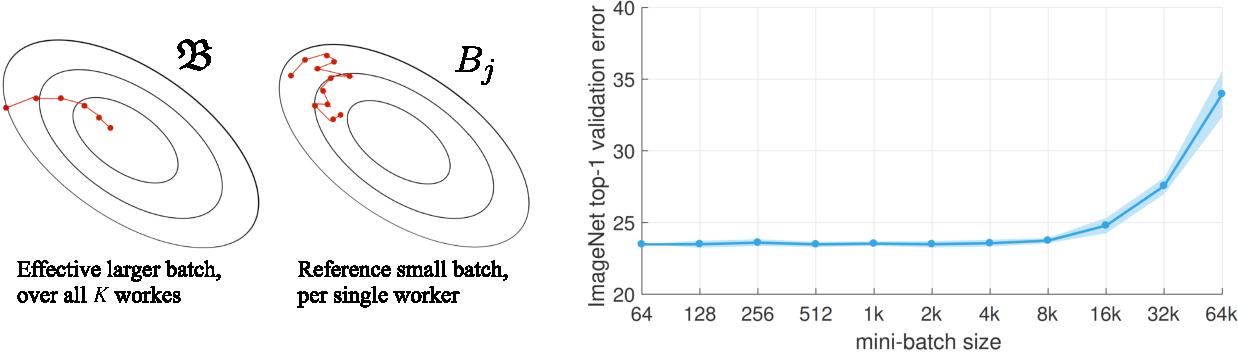
\includegraphics[width=0.8\textwidth]{../images/Effective_Reference_Batch_ImageNet_Goyal_2.pdf}}

\footnote<.->{\tiny Goyal et al, 2017}
\end{frame}

\begin{frame}{Distributed Training on Large Data}
\protect\hypertarget{distributed-training-on-large-data-11}{}
\begin{itemize}
\tightlist
\item
  Efficient Distributed Training with
  \(\vert \mathfrak{B} \vert = K \cdot \vert B_{\text{ref}} \vert\), for
  large \(K\)
\item
  Hyperparameters tuning may allow for even larger batch sizes while
  still reducing time to accuracy
\end{itemize}

\center{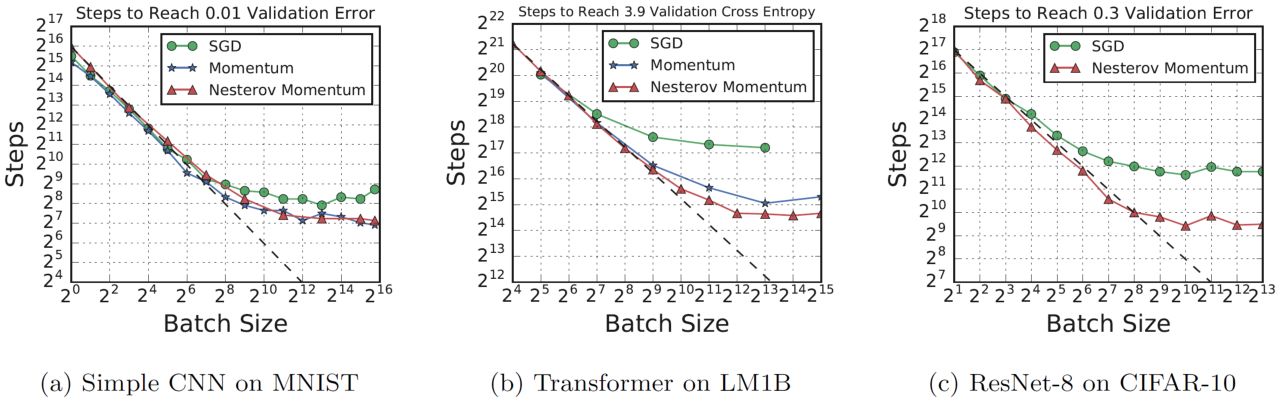
\includegraphics[width=\textwidth]{../images/Batch_Size_Critical_Different_Optimizers.pdf}}

\footnote<.->{\tiny Shallue et al, JMLR, 2019}
\end{frame}

\begin{frame}{Distributed Training on ImageNet}
\protect\hypertarget{distributed-training-on-imagenet}{}
\begin{itemize}
\tightlist
\item
  Efficient Distributed Training with
  \(\vert \mathfrak{B} \vert = K \cdot \vert B_{\text{ref}} \vert\), for
  large \(K\)
\item
  Combating accuracy loss when using larger batch sizes: hyperparameter
  tuning
\item
  Reducing \textbf{time to accuracy} with \textbf{target accuracy} equal
  to a working smaller batch (single node) reference
\end{itemize}

\center{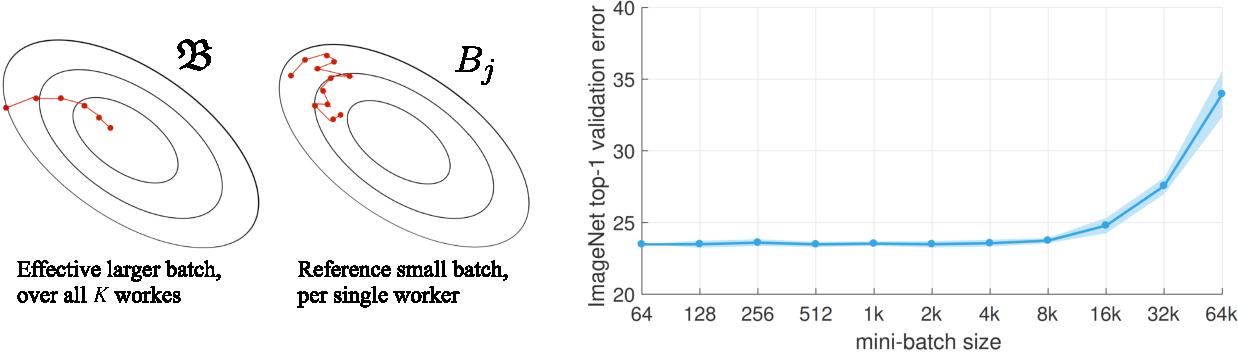
\includegraphics[width=0.8\textwidth]{../images/Effective_Reference_Batch_ImageNet_Goyal_2.pdf}}
\end{frame}

\begin{frame}{Distributed Training on ImageNet}
\protect\hypertarget{distributed-training-on-imagenet-1}{}
\begin{itemize}
\tightlist
\item
  Combating accuracy loss when using larger batch sizes: hyperparameter
  tuning
\item
  Learning rate rescaling with respect to \(\vert \mathfrak{B} \vert\)
  and \(\vert B_{\text{ref}} \vert\)
\end{itemize}

\center{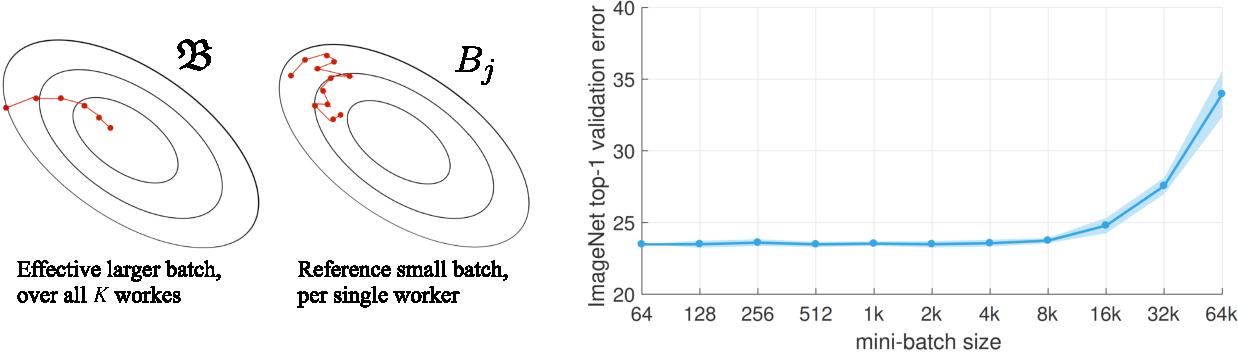
\includegraphics[width=0.8\textwidth]{../images/Effective_Reference_Batch_ImageNet_Goyal_2.pdf}}
\end{frame}

\hypertarget{combating-accuracy-loss-on-imagenet}{%
\section{Combating accuracy loss on
ImageNet}\label{combating-accuracy-loss-on-imagenet}}

\begin{frame}{Combating accuracy loss on ImageNet}
\begin{itemize}
\tightlist
\item
  Learning rate rescaling: motivation to match weight updates for
  different batch sizes \(\vert \mathfrak{B} \vert\),
  \(\vert B_{\text{ref}} \vert\),
  \(\vert \mathfrak{B} \vert = K \cdot \vert B_{\text{ref}} \vert\)
\end{itemize}

\center{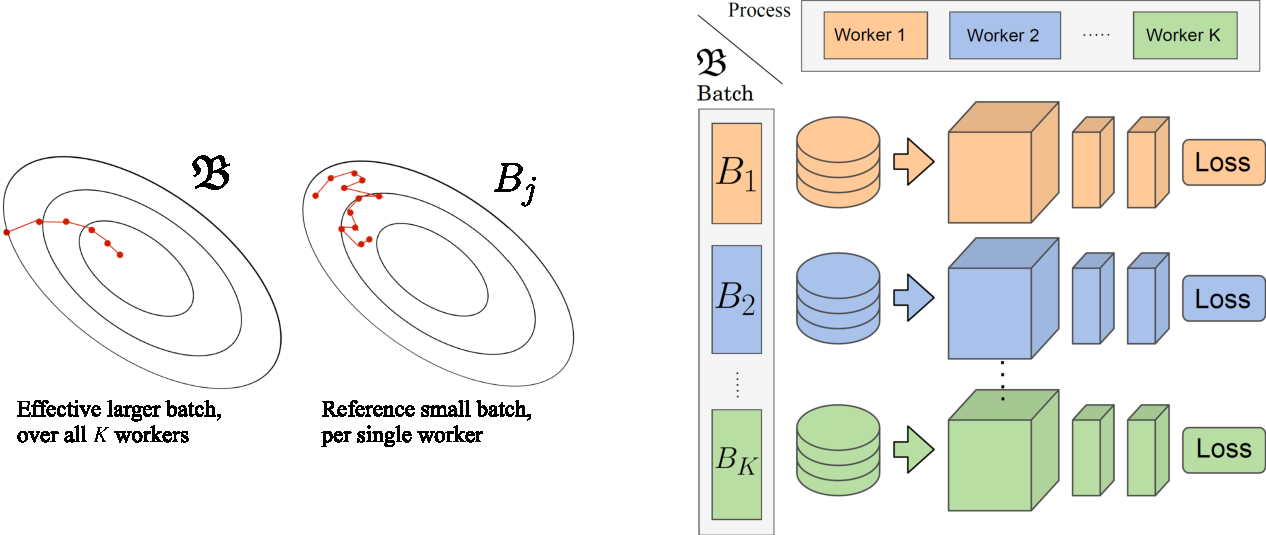
\includegraphics[width=0.8\textwidth]{../images/Large_Small_Reference_Batch_Data_Parallel_Model_Workers_Processes.pdf}}
\end{frame}

\hypertarget{combating-accuracy-loss-on-imagenet-1}{%
\section{Combating accuracy loss on
ImageNet}\label{combating-accuracy-loss-on-imagenet-1}}

\begin{frame}{Combating accuracy loss on ImageNet}
\begin{itemize}
\tightlist
\item
  Learning rate rescaling: motivation to match weight updates for
  different batch sizes,
  \(\vert \mathfrak{B} \vert = K \cdot \vert B_{\text{ref}} \vert\)

  \begin{itemize}
  \tightlist
  \item
    increase the weight update step size to accommodate for the fewer
    number of update steps when having a larger batch size
  \end{itemize}
\end{itemize}

\center{

$K$ update steps of SGD with learning rate $\eta$ and $\vert B_{\text{ref}} \vert = n$:

$$ \mathbf{W}_{t+K} = \mathbf{W}_t - \underbrace{\eta \frac{1}{n}} \sum_{j<K} \sum_{X\in B_j} \nabla \underbrace{\mathcal{L}(X,\mathbf{W}_{t+j})} $$


Single update step with $\vert \mathfrak{B} \vert = Kn$, learning rate $\hat\eta$


$$ \mathbf{\hat W}_{t+1} = \mathbf{W}_t  -  \underbrace{\hat\eta \frac{1}{Kn}} \sum_{j<K} \sum_{X\in B_j} \nabla \underbrace{\mathcal{L}(X,\mathbf{W}_t)} $$
}

\footnote<.->{\tiny Goyal et al, 2017}
\end{frame}

\hypertarget{combating-accuracy-loss-on-imagenet-2}{%
\section{Combating accuracy loss on
ImageNet}\label{combating-accuracy-loss-on-imagenet-2}}

\begin{frame}{Combating accuracy loss on ImageNet}
\begin{itemize}
\tightlist
\item
  Learning rate: linear rescaling, \(\hat\eta = K \eta\), for
  \(\vert \mathfrak{B} \vert = K \cdot \vert B_{\text{ref}} \vert\)
\end{itemize}

\vspace*{0.5cm}

\center{

To get $\mathbf{\hat W}_{t+1} \approx \mathbf{W}_{t+K}$,

\vspace*{0.5cm}

we assume $\nabla \mathcal{L}(X,\mathbf{W}_t) \approx \nabla \mathcal{L}(X,\mathbf{W}_{t+j})$ for $j<K$

and obtain $$ \hat\eta \tfrac{1}{kn} = \eta \tfrac{1}{n} \Leftrightarrow \hat\eta = \tfrac{kn}{n} \eta \Leftrightarrow \hat\eta = K \eta $$

}

\footnote<.->{\tiny Goyal et al, 2017}
\end{frame}

\begin{frame}{Combating accuracy loss on ImageNet}
\protect\hypertarget{combating-accuracy-loss-on-imagenet-3}{}
\begin{itemize}
\tightlist
\item
  Learning rate: linear rescaling, \(\hat\eta = K \eta\), for
  \(\vert \mathfrak{B} \vert = K \cdot \vert B_{\text{ref}} \vert\)

  \begin{itemize}
  \tightlist
  \item
    used in combination with usual learning rate schedules
  \end{itemize}
\item
  \(\nabla \mathcal{L}(X,\mathbf{W}_t) \approx \nabla \mathcal{L}(X,\mathbf{W}_{t+j})\)
  for \(j<K\) does not hold in general

  \begin{itemize}
  \tightlist
  \item
    especially wrong for initial learning phase where gradients vary a
    lot from step to step
  \item
    A possible remedy: initial warm-up phase
  \end{itemize}
\end{itemize}

\center{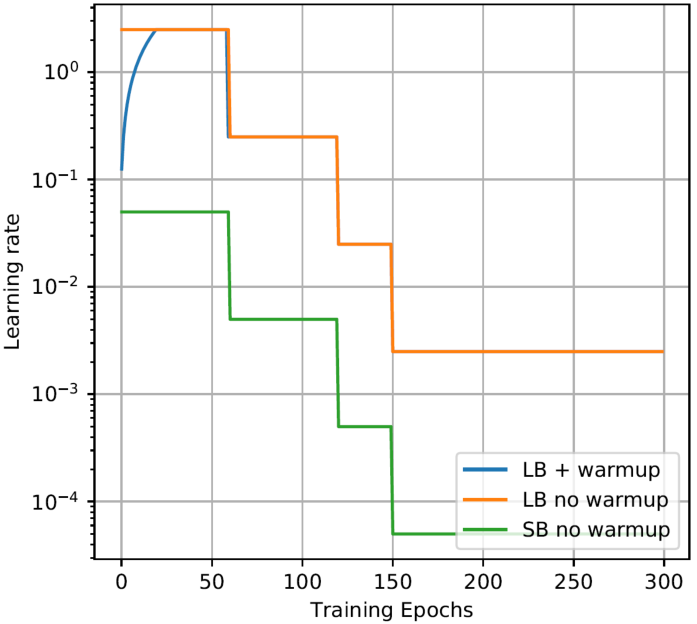
\includegraphics[width=0.45\textwidth]{../images/WarmUp_LearningRate_Schedules.pdf}}
\end{frame}

\begin{frame}{Combating accuracy loss on ImageNet}
\protect\hypertarget{combating-accuracy-loss-on-imagenet-4}{}
\begin{itemize}
\tightlist
\item
  Learning rate: linear rescaling, \(\hat\eta = K \eta\), for
  \(\vert \mathfrak{B} \vert = K \cdot \vert B_{\text{ref}} \vert\)

  \begin{itemize}
  \tightlist
  \item
    used in combination with usual learning rate schedules
  \end{itemize}
\item
  \(\nabla \mathcal{L}(X,\mathbf{W}_t) \approx \nabla \mathcal{L}(X,\mathbf{W}_{t+j})\)
  for \(j<K\) is bad assumption for early learning
\item
  Warm-up phase: start with \(\eta\), increase towards scaled
  \(\hat\eta = K \eta\) within few epochs
\end{itemize}

\center{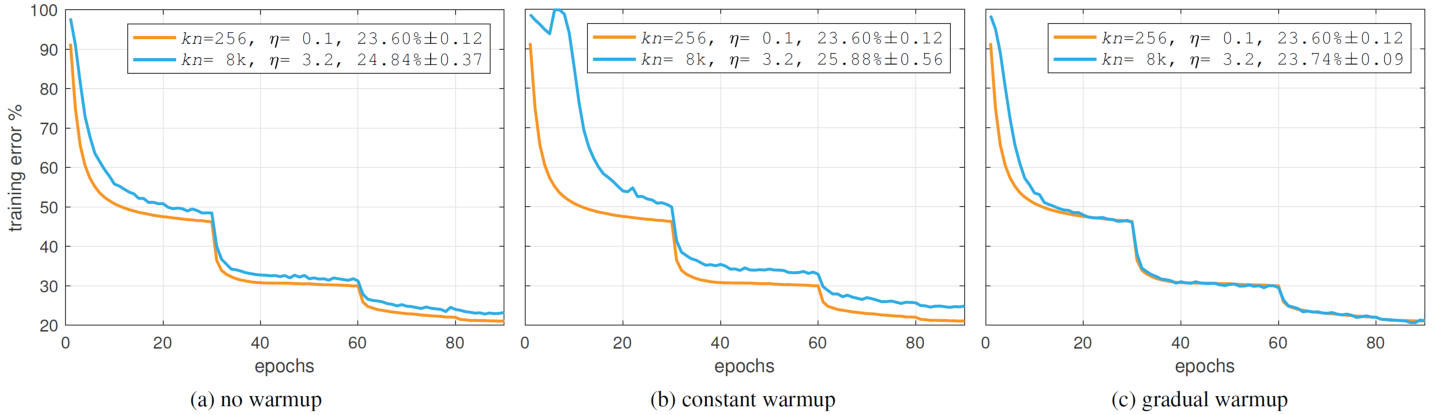
\includegraphics[width=\textwidth]{../images/WarmUp_BatchSizes_ResNet_ImageNet_Goyal.pdf}}

\footnote<.->{\tiny Goyal et al, 2017}
\end{frame}

\begin{frame}{Combating accuracy loss on ImageNet}
\protect\hypertarget{combating-accuracy-loss-on-imagenet-5}{}
\begin{itemize}
\tightlist
\item
  Learning rate tuning: package of mechanisms

  \begin{itemize}
  \tightlist
  \item
    linear rescaling
  \item
    Warm-up for initial epochs
  \item
    Schedules
  \end{itemize}
\end{itemize}

\center{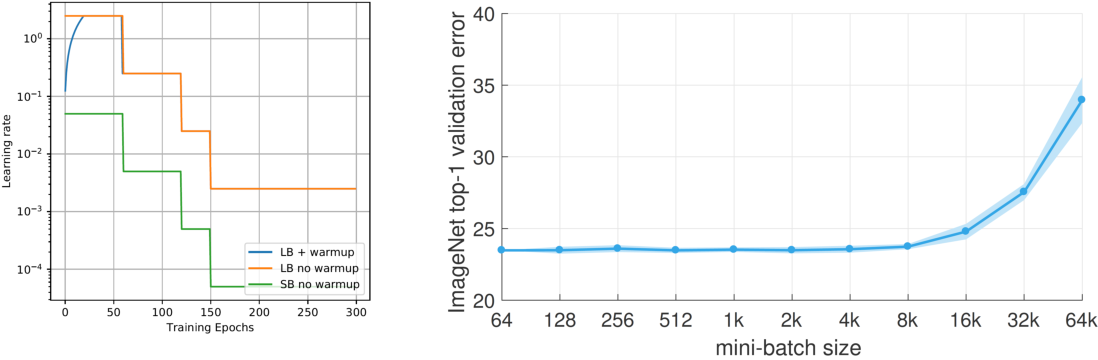
\includegraphics[width=\textwidth]{../images/Learning_Rate_Schedule_Package_ImageNet_8k_Goyal}}
\end{frame}

\begin{frame}{Combating accuracy loss on ImageNet}
\protect\hypertarget{combating-accuracy-loss-on-imagenet-6}{}
\begin{itemize}
\tightlist
\item
  Learning rate tuning: package of mechanisms
\item
  Often, still not enough for very large batch sizes
  \(\vert \mathfrak{B} \vert > 8192\)
\item
  Advanced Optimizers that provide further adaptive hyperparamer tuning
  during training
\end{itemize}

\center{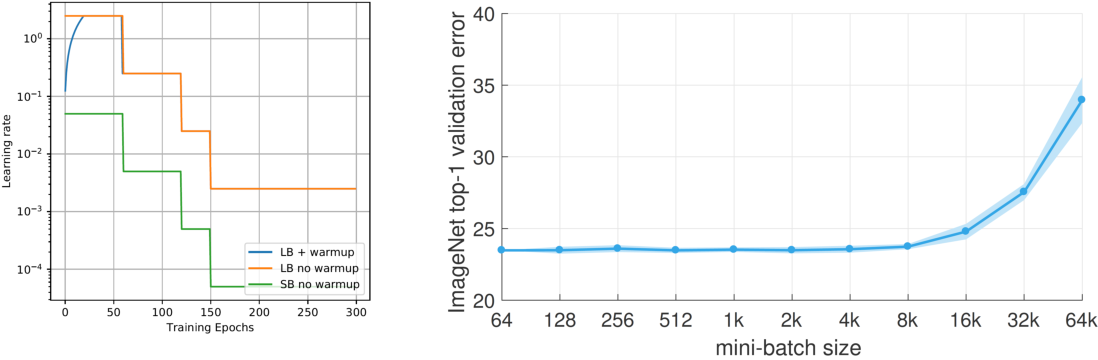
\includegraphics[width=\textwidth]{../images/Learning_Rate_Schedule_Package_ImageNet_8k_Goyal.pdf}}
\end{frame}

\begin{frame}{Combating accuracy loss on ImageNet}
\protect\hypertarget{combating-accuracy-loss-on-imagenet-7}{}
\begin{itemize}
\tightlist
\item
  Advanced optimizers that provide further adaptive hyperparamer tuning
  during training: very large batch sizes
  \(\vert \mathfrak{B} \vert > 8192\)
\item
  LARS : Layer-wise Adaptive Rate Scaling, extension of SGD with
  momentum

  \begin{itemize}
  \tightlist
  \item
    tuning learning rates layerwise depending on gradient and weight
    amplitudes and norms
  \end{itemize}
\item
  LAMB : Layer Adaptive Moment Batch, extension of LARS (use AdamW as
  base)

  \begin{itemize}
  \tightlist
  \item
    tuning learning rate layerwise, also per weight parameter using
    gradient mean and variance
  \end{itemize}
\end{itemize}

\center{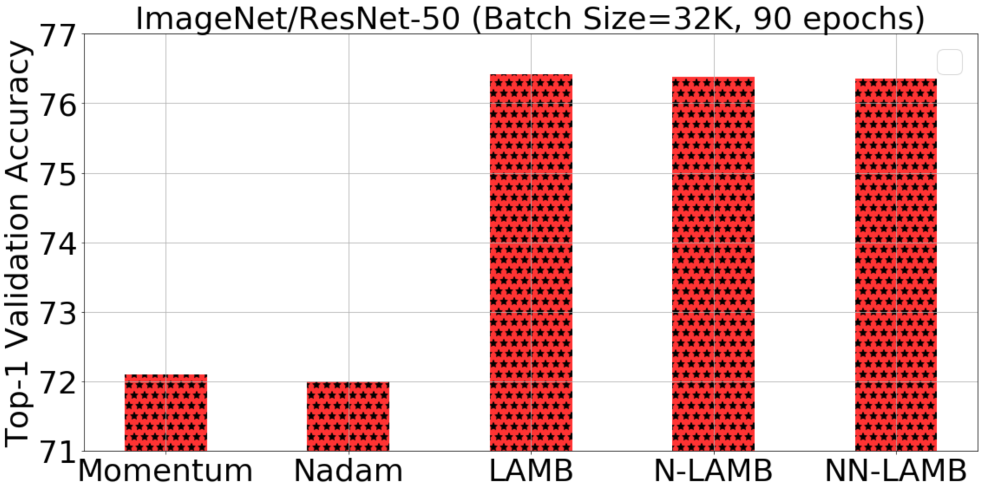
\includegraphics[width=0.45\textwidth]{../images/LAMB_32k_ResNet_ImageNet.pdf}}

\footnote<.->{\tiny You et al, ICLR, 2020}
\end{frame}

\begin{frame}{Combating accuracy loss on ImageNet}
\protect\hypertarget{combating-accuracy-loss-on-imagenet-8}{}
\begin{itemize}
\tightlist
\item
  Learning rate rescaling, schedules and Warm up : works well for
  \(\vert \mathfrak{B} \vert \leq 8192\))
\item
  Advanced optimizers (LAMB) : works for
  \(\vert \mathfrak{B} \vert \leq 80k\))
\item
  Almost linear speed-up in training time without accuracy loss:
  reducing \textbf{time to accuracy}
\end{itemize}

\center{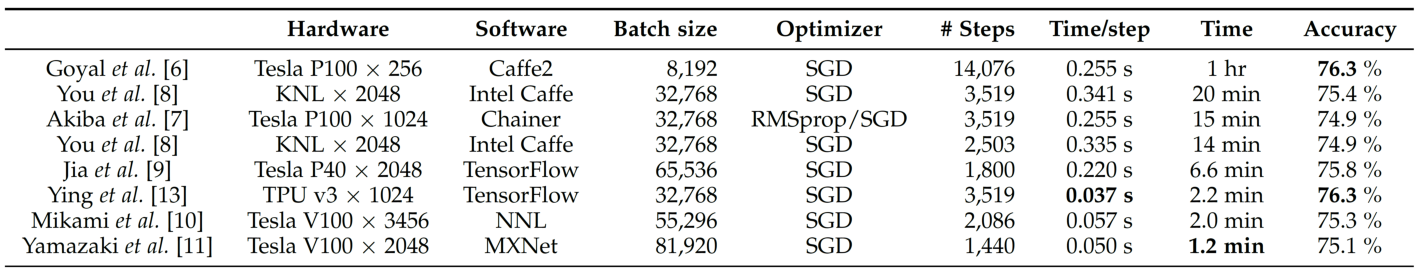
\includegraphics[width=\textwidth]{../images/Table_ImageNet_Training_BatchSizes.pdf}}

\footnote<.->{\tiny Osawa et al, 2020}
\end{frame}

\begin{frame}{Distributed training with large batches}
\protect\hypertarget{distributed-training-with-large-batches}{}
\begin{itemize}
\tightlist
\item
  More advanced techniques may allow efficient distributed training
  beyond batch size issues\\
\item
  Local SGD: giving up consistency between model parameters across
  different workers after each update
\item
  Post Local SGD: combining coupled global SGD and decoupled local SGD
\item
  Natural SGD: attempt to use second derivatives and curvature
  information
\end{itemize}

\center{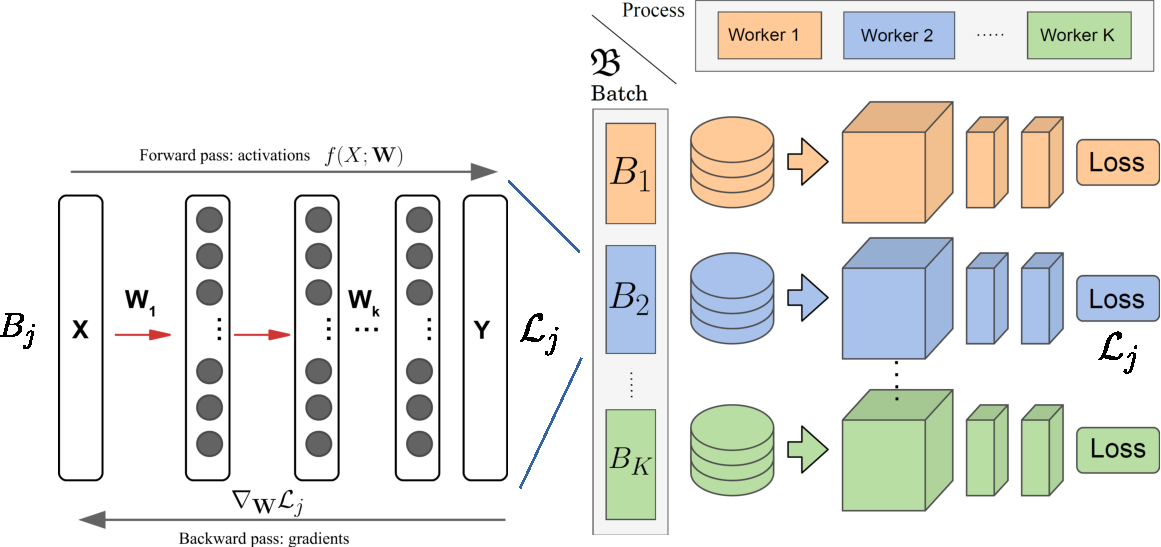
\includegraphics[width=0.8\textwidth]{../images/Forward_Backward_Data_Parallel_Workers_Batches.pdf}}
\end{frame}

\begin{frame}{Distributed training with large batches}
\protect\hypertarget{distributed-training-with-large-batches-1}{}
\begin{block}{Summary}
\protect\hypertarget{summary}{}
\begin{itemize}
\tightlist
\item
  Efficient data parallel training on large datasets like ImageNet-1k
\item
  Measures to stabilize training with large batches necessary
\item
  Learning rate scaling, schedules, warm-up phase, specialized
  optimizers
\item
  Advanced methods required for very large
  \(\vert \mathfrak{B} \vert \geq 32k\)
\item
  Aim: reduce \textbf{time to accuracy} without accuracy loss
\end{itemize}
\end{block}

\center{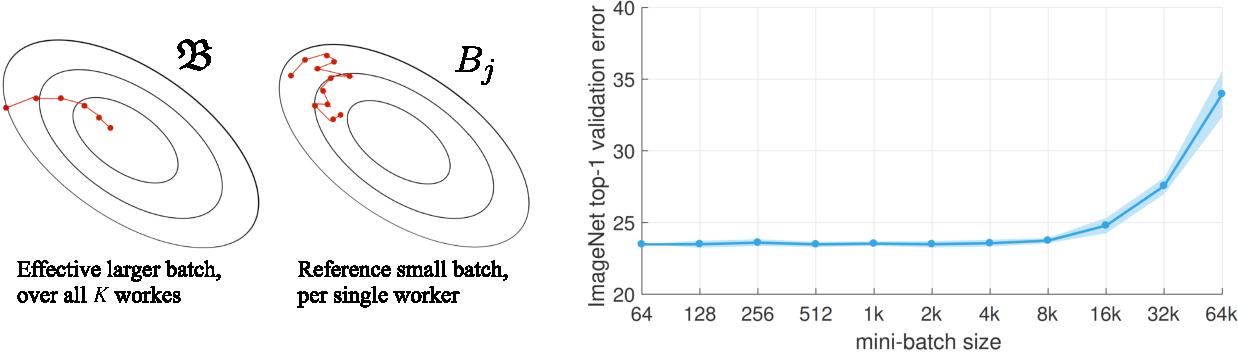
\includegraphics[width=0.8\textwidth]{../images/Effective_Reference_Batch_ImageNet_Goyal_2.pdf}}
\end{frame}


\end{document}
